\subsection{SpaceTime}
\label{ssec:spacetime}

\emph{SpaceTime} (or Serenity Mark I) was the title given to the most advanced Haskell prototype developed. The concept, inspired by the RTS game \emph{Achron},\sidenote[][1em]{http://www.achrongame.com/site/} explores the concept of a game where past actions can be changed, affecting the present and future. This concept formed the early ideas that grew into the full Project Serenity design, although the time travel aspect was eventually dropped.

SpaceTime prototyped several concepts that were later refined in Project Serenity, including a basic framework for AI and a system for button widgets for giving commands. Player actions were modelled as happening at the specific moment selected in the timeline (see screenshot in Figure~\ref{fig:spacetimescreen}), which could be dragged to a different position or played at a constant rate and the current version of events would animate. If a new command is given at a specific point then history is recalculated.

\begin{figure}
	\caption[A screen from \emph{SpaceTime}][2em]{A screen capture from \emph{SpaceTime}.}
	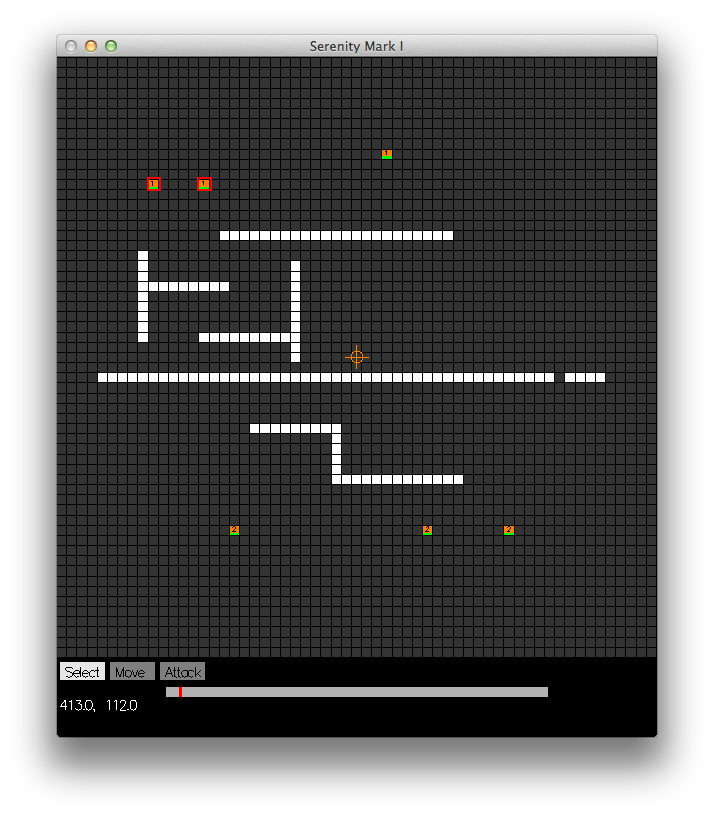
\includegraphics[width=29em]{res/spacetime/spacetimescreen.png}
	\label{fig:spacetimescreen}
\end{figure}

A problem encountered during the development of SpaceTime was the effect of lazy evaluation on frame rate. The lazy semantics of Haskell are highly beneficial in most ways, but can in some cases lead to problems. Evaluation can be forced, but the best way to do so is not always obvious. The prelude provides a function "seq", which fully evaluates its first argument before returning its second. However, there are many pitfalls for the unwary. For example, the expression "seq a a" is actually equivalent to just "a", and so evaluation is not forced. Also, the forced evaluation is only to \emph{weak head normal form} (WHNF). This is a technical term and the details are out of the scope of this discussion,\sidenote{For more details on WHNF see \url{en.wikibooks.org/wiki/Haskell/Graph_reduction}.} but the main repercussion of this is that if "seq" is used to force a list, only the first element will actually be evaluated. Further tricks are required to force each element of the list to WHNF (this is referred to as forcing the \emph{spine} of the list). Forcing evaluation of the length of the list will force the spine for example. There is a package called \emph{deepseq} to help address these issues, but they can still be hard to identify and fix.

The SpaceTime prototype was invaluable in many ways to the later development of the full Project Serenity. Most notably it taught that good structuring of Haskell modules is not as obvious as first impressions might suggest, and that some thought at the beginning of a project can go a long way. Given the problems with laziness, it was suspected that similar issues might crop up in the full game, but this didn't actually happen. SpaceTime also highlighted the complexities of user interface programming with Gloss, that led eventually to the development of the Sheen framework (see Section~\ref{sec:gui}).
